\chapter{Spherical samples}
\label{ch:sphere}

\section{The idea}

Version~2.4 adds a fourth geometry: \textbf{concentric spheres} (Figure~\ref{fig:sphere}). The sample is a full sphere surrounded by
spherical shells, like an onion: a powder ball in a thin spherical container, a droplet, a single-crystal sphere, a ball of one
material, or a spherical flask partly filled with a liquid.

\begin{itemize}
  \item The common \textbf{centre} of the spheres is the centre of the instrument, on the beam axis ($x=y=z=0$).
  \item The layers are given \textbf{from the inner one outwards}, exactly as for the cylinder: the thickness of the first layer is its
        \textbf{diameter}, and the thickness of every other layer is the \textbf{radial thickness} of its shell,
        \begin{equation}
          r_1 = t_1/2, \qquad r_k = r_{k-1} + t_k \quad (k\ge2).
        \end{equation}
        For instance the thicknesses $(6.0,\,1.0,\,0.5)$~mm give the radii $(3.0,\,4.0,\,4.5)$~mm and an outer diameter of 9~mm.
  \item Every other property of a layer is the same as in the other geometries: label, $\mu$, scatter fraction, and the vertical extent
        of its material (\code{bottom} and \code{height}, Chapter~\ref{ch:partial}).
  \item A sphere looks the same from every direction: there is \textbf{no orientation} parameter, and the sample frame is the lab frame.
\end{itemize}

\begin{figure}[H]
  \centering
  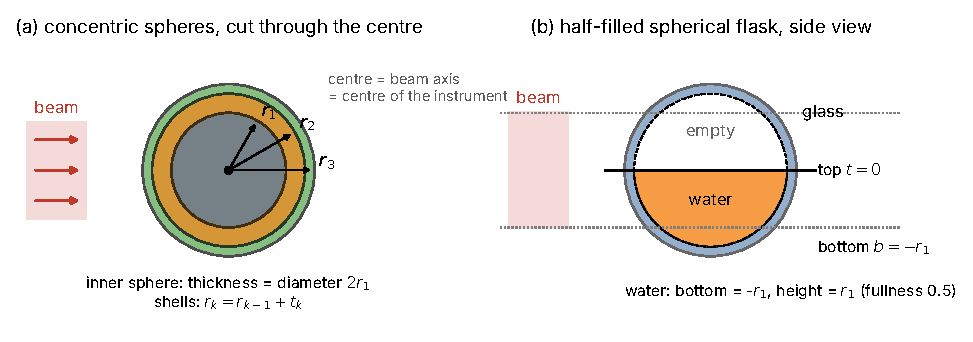
\includegraphics[width=\textwidth]{fig_sphere_geometry}
  \caption{Spherical geometry. (a)~Three concentric spheres cut through their centre, with the radii $r_1<r_2<r_3$; the cut looks the
  same in every plane through the centre. (b)~A spherical flask half filled with water: the glass shell is full, the inner sphere has
  water from its bottom ($y=-r_1$) up to $y=0$, the centre of the beam.}
  \label{fig:sphere}
\end{figure}

\section{Geometry and conventions}

Layer $i$ occupies the shell $r_{i-1} \le |\vec r| \le r_i$ ($r_0=0$), and its material the part of the shell with
$b_i \le y \le t_i$:
\begin{equation}
  r_{i-1} \le \sqrt{x^2+y^2+z^2} \le r_i, \qquad b_i \le y \le t_i .
\end{equation}
\begin{description}
  \item[Vertical extent.] The sample goes from $y=-R_\mathrm{out}$ to $y=+R_\mathrm{out}$ ($y_\mathrm{bottom} = -R_\mathrm{out}$,
        height $2R_\mathrm{out}$). The bands of the layers are cut at the outer sphere. In the forms of version~2.0, \code{fill_height}
        is measured from the lowest point of the sphere, and \code{fullness} from the bottom of the beam.
  \item[Fullness.] \code{beam_fullness()} is the fraction of the beam \emph{height} covered by the band of the material, as for the
        other geometries. For a sphere the illuminated width changes with the height, so it is a fraction of height, not of
        material.
  \item[Detector.] Because of the symmetry, the transmission towards a detector depends only on the angle between the detector and
        the beam, not on the azimuth $\varphi$, as long as the beam illuminates the sphere symmetrically (beam larger than the sphere, or
        square and centred). With a partially filled layer or a rectangular beam smaller than the sphere this symmetry is lost.
\end{description}

\begin{note}[Sphere and cylinder]
In the horizontal plane a sphere and a cylinder of the same radius look alike: both are circles. The difference is vertical. A
particle scattered in a cylinder at height $y$ towards a detector in the horizontal plane crosses a circle of radius $R$; in a sphere it
crosses a circle of radius $\sqrt{R^2-y^2}$, smaller away from the centre. The paths are therefore shorter, the attenuation smaller, and
it changes less with the angle (Section~\ref{sec:sphere-results}).
\end{note}

\section{Creating a spherical sample}

\begin{fnbox}{create\_spherical\_sample(layers, beam\_height=None)}
\code{layers}: from the inner sphere outwards; tuples, dictionaries or \code{Layer} objects, as for the other geometries. The first
thickness is the diameter of the inner sphere, the others radial thicknesses. \code{beam_height}: height of the beam (mm), needed for
\code{fullness} and \code{beam_fullness()}. Returns a \code{SphericalSample}.
\end{fnbox}

\begin{lstlisting}
from sphere import create_spherical_sample
from sample_base import Layer

ball = create_spherical_sample([("Ni", 6.0, 0.180, 0.94),     # inner sphere: diameter 6 mm
                                ("V",  0.2, 0.046, 0.78)])    # container: wall 0.2 mm
flask = create_spherical_sample([Layer("water", 20.0, 0.56, 1.0, bottom=-10.0, height=10.0),
                                 ("glass", 1.0, 0.03, 1.0)], beam_height=8.0)
\end{lstlisting}
With the factory the geometry is \code{"sphere"} (also \code{"spherical"} or \code{"ball"}). Nothing else is needed: the size comes from
the thicknesses, and \code{height}, \code{width}, \code{y_bottom} and \code{plane_angle_deg} are not used.
\begin{lstlisting}
from sample_factory import make_sample
sample = make_sample("sphere", layers, beam_height=8.0)
\end{lstlisting}

\section{What the spherical sample tells you}

\begin{center}\small
\begin{tabular}{@{}>{\raggedright\arraybackslash}p{6.1cm}p{8.7cm}@{}}
  \toprule \textbf{Attribute or method} & \textbf{Content} \\ \midrule
  \code{sample.radii}, \code{sample.inner_radii} & outer and inner radius of each layer (mm) \\
  \code{sample.outer_radius}, \code{sample.diameter} & $R_\mathrm{out}$ and $2R_\mathrm{out}$ (mm) \\
  \code{sample.summary()} & table of the layers: radii, thickness, $\mu$, scatter fraction, band of the material and fullness \\
  \code{sample.section_area_in_beam(w_b, h_b)} & area (mm$^2$) of the part of a uniform $w_b\times h_b$ beam that meets the sphere (the circle of radius $R_\mathrm{out}$ inside the beam rectangle). Divided by $w_b h_b$ it is the fraction of the beam that meets the sample; $\pi R_\mathrm{out}^2$ for a beam larger than the sphere. \\
  \code{sample.y_bottom}, \code{sample.y_top} & $-R_\mathrm{out}$ and $+R_\mathrm{out}$ \\
  \code{sample.contains(p)} & True for the points with $|\vec r|\le R_\mathrm{out}$ \\
  \code{sample.layer_of_points(p)} & layer from the distance to the centre; $-1$ outside, or in the empty part of a layer \\ \bottomrule
\end{tabular}
\end{center}
The section area is
\begin{equation}
  S = \int_{|y| < \min(R_\mathrm{out},\,h_b/2)} \min\!\left(2\sqrt{R_\mathrm{out}^2-y^2},\; w_b\right) \deriv{y},
\end{equation}
computed by the trapezoidal rule on a fine grid.

\section{Example}

\pyexample{ex12_sphere}

The beam ($8\times8$~mm) is larger than the sphere (6.4~mm): only half of it meets the sample ($\pi\,3.2^2/64 = 0.503$). The
transmission is lowest at $0^\circ$ and highest at $180^\circ$, as for a cylinder, but it changes less with the angle. Towards a detector in
the vertical plane ($\varphi=90^\circ$) the transmission is the same as in the horizontal plane, within the statistics: the sphere has no
preferred direction and the square beam illuminates it symmetrically. The flask has water from $y=-10$ to $0$~mm, i.e.\ the lower half
of the 8~mm beam (fullness 0.5).

\section{How it is computed}
\label{sec:sphere-algorithm}

The cylinder cuts every straight path $\vec p + s\,\hat d$ into \emph{segments}, at every place where the material may change: where it
crosses the boundary of a layer, and where it crosses one of the horizontal planes that limit the material of the partially filled
layers. Inside one segment the material is always the same; the layer is found from the distance of the midpoint of the segment to the
axis, and whether it is material or empty space from the height of the midpoint. The path in each layer and the next interaction
follow by walking along the segments (Chapter~\ref{ch:physics}).

The sphere uses exactly the same procedure with three changes:
\begin{enumerate}
  \item \textbf{Crossings of a layer boundary.} A point of the path is on the sphere of radius $r_i$ when $|\vec p + s\,\hat d|^2 = r_i^2$,
        \begin{equation}
          a\,s^2 + 2b\,s + c = 0, \qquad a = \hat d\cdot\hat d = 1,\quad b = \vec p\cdot\hat d,\quad c = |\vec p|^2 - r_i^2,
        \end{equation}
        with the two solutions $s_\pm = (-b \pm \sqrt{b^2 - ac})/a$, where the path enters and leaves the sphere. If $b^2-ac\le0$ it misses
        it. Unlike the cylinder there is no special direction (for the cylinder, a vertical path never crosses the side surface).
  \item \textbf{The layer of a point} is given by its distance to the \emph{centre}, $\sqrt{x^2+y^2+z^2}$, instead of its distance to
        the vertical axis.
  \item \textbf{The outline} of the sample is the outer sphere: there are no flat ends.
\end{enumerate}
In the code, \code{CylindricalSample} computes these three things in three small methods, \code{_shell_interval}, \code{_radius_of} and
\code{_outline_interval}, and \code{SphericalSample}, a subclass of \code{CylindricalSample}, redefines them:
\begin{lstlisting}
class SphericalSample(CylindricalSample):
    @staticmethod
    def _radius_of(x, y, z):
        return np.sqrt(x * x + y * y + z * z)            # distance to the centre

    def _shell_interval(self, p, d, R):
        a = np.sum(d * d, axis=1)
        b = np.sum(p * d, axis=1)
        c = np.sum(p * p, axis=1) - R * R
        disc = b * b - a * c
        crosses = disc > 0.0
        root = np.sqrt(np.where(crosses, disc, 0.0))
        return (np.where(crosses, (-b - root) / a, np.inf),
                np.where(crosses, (-b + root) / a, -np.inf))

    def _outline_interval(self, p, d):
        return self._shell_interval(p, d, self.outer_radius)
\end{lstlisting}
It also redefines \code{contains}, \code{summary} and the constructor (the vertical extent follows from the outer radius), and adds
\code{section_area_in_beam}. Everything else (interaction points, path lengths, next interaction, multiple scattering, direct method) is
inherited. The cylinder itself was only reorganised: its results are bit-for-bit those of version~2.3 (Chapter~\ref{ch:validation}).

\section{Results}
\label{sec:sphere-results}

The figures of this section use the example layers of the main script (\code{SPHERE_LAYERS}: Fe of diameter 6~mm, Al 1~mm, Cu 0.5~mm,
the same as the example cylinder) and a beam of $8\times8$~mm, which is smaller than the sphere (outer diameter 9~mm).

\begin{figure}[H]
  \centering
  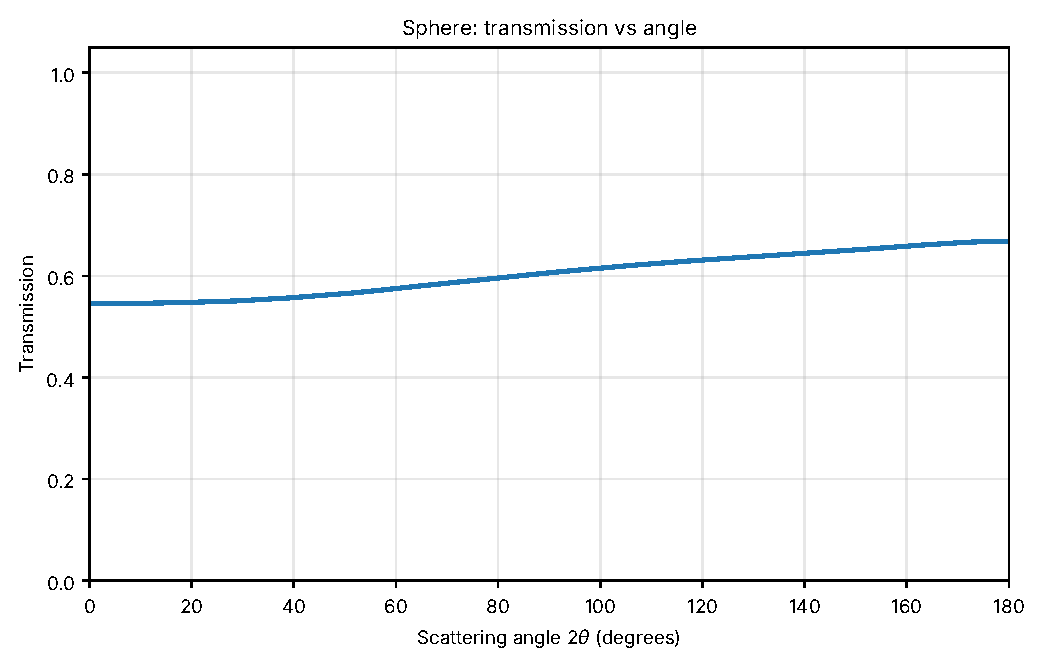
\includegraphics[width=0.78\textwidth]{fig_transmission_sphere}
  \caption{Example sphere: transmission of the singly scattered particles versus $\twotheta$ ($5\times10^4$ particles).}
  \label{fig:transsphere}
\end{figure}

\begin{figure}[H]
  \centering
  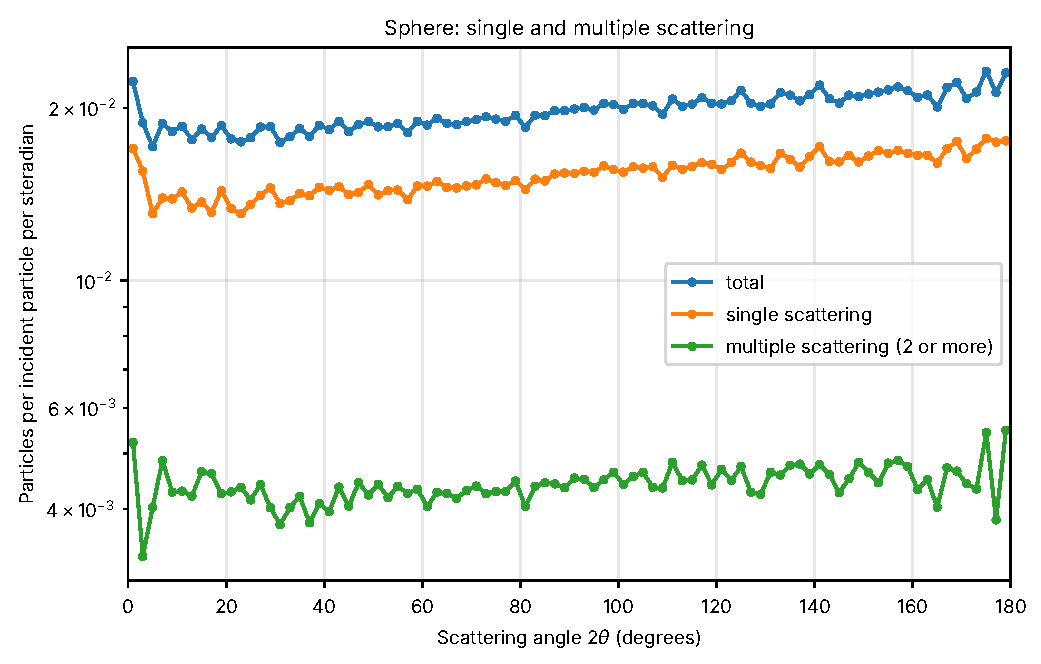
\includegraphics[width=0.78\textwidth]{fig_orders_sphere}
  \caption{Example sphere: single and multiple scattering per steradian, $10^6$ incident particles.}
  \label{fig:orderssphere}
\end{figure}

\begin{figure}[H]
  \centering
  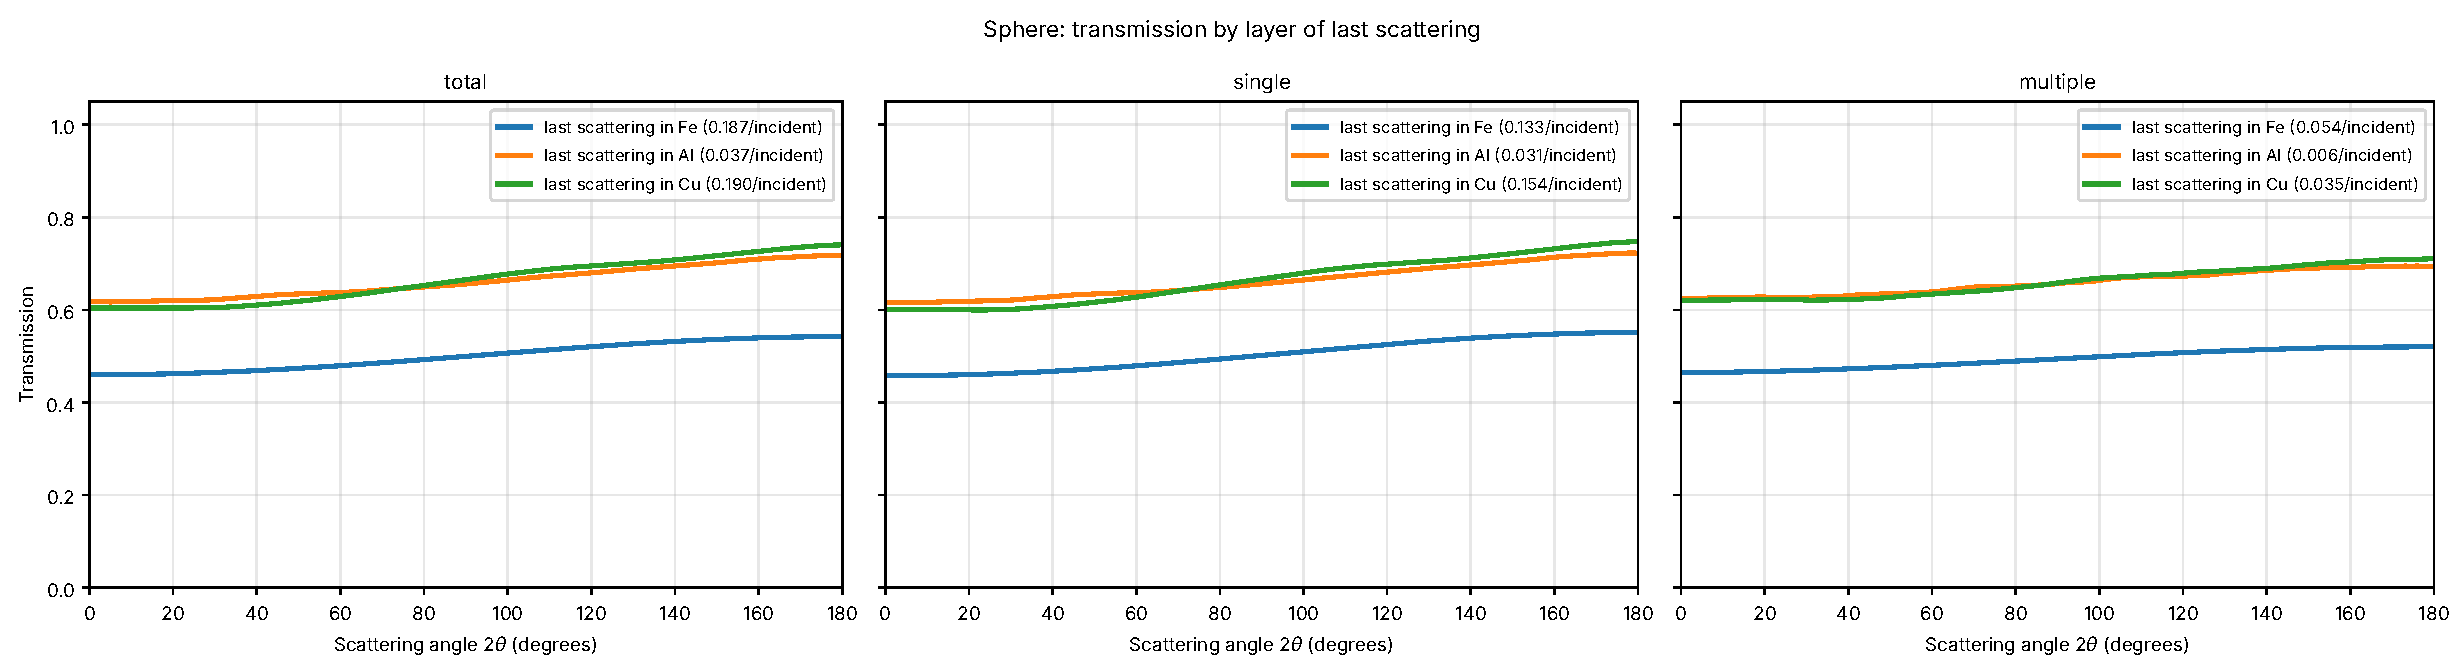
\includegraphics[width=\textwidth]{fig_bylayer_sphere}
  \caption{Example sphere: transmission by layer of last scattering (Chapter~\ref{ch:lastlayer}).}
  \label{fig:bylayersphere}
\end{figure}

\paragraph{Sphere or cylinder?} Figure~\ref{fig:spherevscyl} compares the single-scattering attenuation factor $A(\twotheta)$ (the
Paalman \& Pings factor, computed with the direct method of Chapter~\ref{ch:direct}) of a homogeneous sphere and of a long cylinder
of the same radius (3~mm), for $\mu R=0.5$, 1 and 2, with a beam larger than both.
\begin{itemize}
  \item The sphere attenuates less: $A(0) = 0.483$, 0.242 and 0.071 against 0.434, 0.196 and 0.047 for the cylinder. Its mean chord,
        $4R/3$, is shorter than that of the cylinder, $\pi R/2$.
  \item The attenuation of the sphere changes less with the angle: $A(180^\circ)/A(0)$ is 1.10, 1.37 and 2.52 for the sphere, against
        1.12, 1.50 and 3.31 for the cylinder.
  \item These values can be compared with the tabulated absorption corrections $A^* = 1/A$ for spheres and cylinders
        (\emph{International Tables for Crystallography}, Vol.~C): at $\mu R=1$ and $\twotheta=0$, $A^* = 4.13$ for the sphere and
        $5.10$ for the cylinder here.
\end{itemize}

\begin{figure}[H]
  \centering
  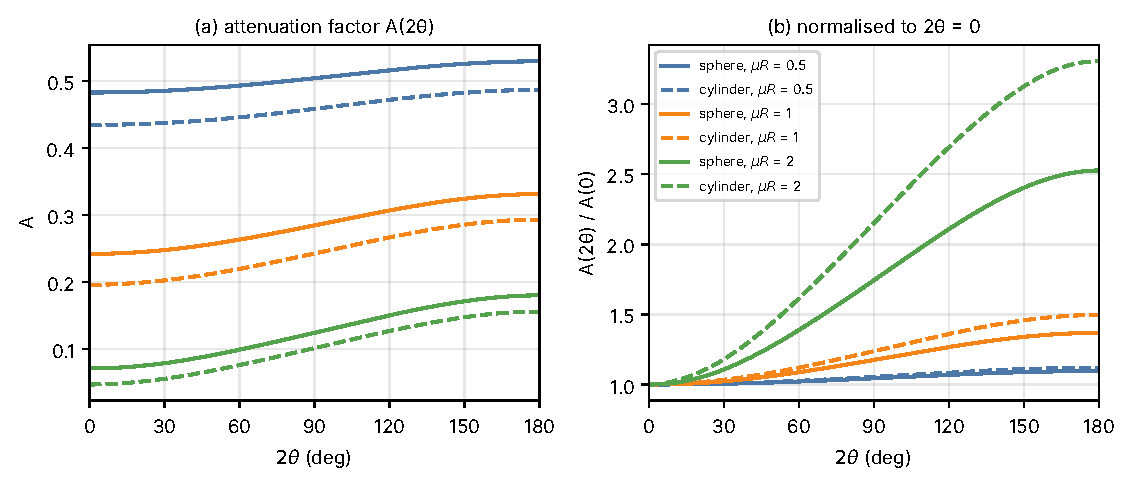
\includegraphics[width=\textwidth]{fig_sphere_vs_cylinder}
  \caption{Attenuation factor of a homogeneous sphere (solid lines) and of a long cylinder (dashed) of radius 3~mm, beam
  $8\times8$~mm, direct method with $6\times10^4$ points, every $1^\circ$. (a)~$A(\twotheta)$. (b)~The same divided by $A(0)$.}
  \label{fig:spherevscyl}
\end{figure}

\paragraph{Validation.} Figure~\ref{fig:spherevalid} compares the fraction of a beam larger than the sphere that interacts in it
with the exact value. A beam line at distance $s$ from the centre crosses a chord $L = 2u$, $u = \sqrt{R^2-s^2}$; with the area element
$2\pi s\,\deriv s = 2\pi u\,\deriv u$,
\begin{equation}
  P_\mathrm{int} = \frac{2\pi}{w_b h_b}\int_0^R \left(1-\e^{-2\mu u}\right) u\,\deriv u .
\end{equation}
The other checks are listed in Chapter~\ref{ch:validation}.

\begin{figure}[H]
  \centering
  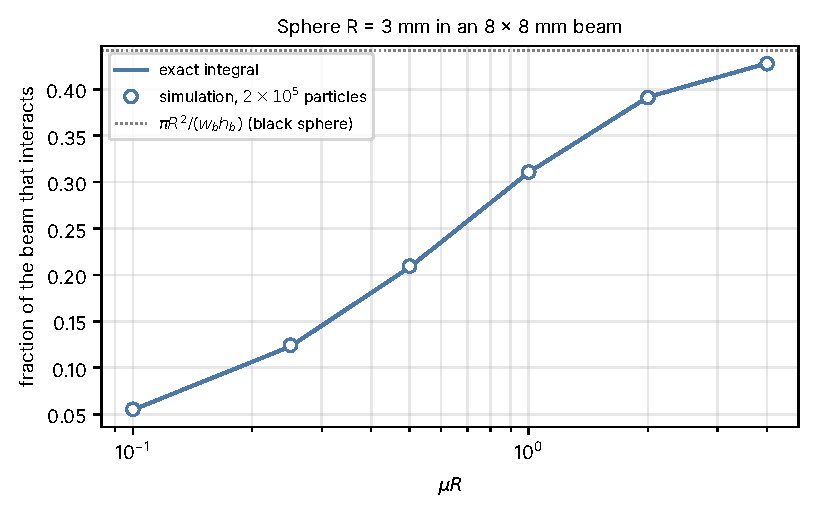
\includegraphics[width=0.75\textwidth]{fig_sphere_validation}
  \caption{Homogeneous sphere of radius 3~mm in an $8\times8$~mm beam: fraction of the beam that interacts, simulation (points) and
  exact integral (line), versus $\mu R$. For large $\mu R$ every particle that meets the sphere interacts: the fraction tends to
  $\pi R^2/(w_bh_b)$ (dotted).}
  \label{fig:spherevalid}
\end{figure}

\section{With the other modules and the main script}

The analysis functions accept a sphere as any other sample:
\begin{itemize}
  \item \code{transmission_vs_angle} (Chapter~\ref{ch:transmission});
  \item \code{simulate_scattering_orders} (Chapter~\ref{ch:scattering});
  \item \code{transmission_by_last_layer} (Chapter~\ref{ch:lastlayer});
  \item \code{attenuation_factors_direct} and the other functions of the direct method (Chapter~\ref{ch:direct}).
\end{itemize} The main script has the geometry \code{sphere}, with the layers \code{SPHERE_LAYERS} set at the
top of \file{run\_simulation.py}; \code{--bottom}, \code{--height} and \code{--fullness} work as for the other geometries
(\code{--plane-angle} is ignored):
\begin{lstlisting}[style=shell]
python run_simulation.py --geometry sphere
python run_simulation.py --geometry sphere --bottom -3 --height 3    # inner sphere half filled
\end{lstlisting}

\begin{note}[Spheres and \textsc{correct}]
\textsc{correct} has no spherical geometry. For a sphere, the attenuation factors (direct method or Monte Carlo) and the multiple
scattering (Monte Carlo) of \mcams{} can replace the cylindrical factors of \textsc{correct} in the same subtraction scheme.
\end{note}

\section{Assumptions and limits}

\begin{itemize}
  \item The spheres are \textbf{concentric} and \textbf{centred on the beam}. An offset sphere would need a centre $(x_0,y_0,z_0)$ in
        \code{_shell_interval} and \code{_radius_of}; it is listed among the possible extensions (Chapter~\ref{ch:limits}).
  \item The material of a partially filled layer is limited by \textbf{horizontal planes}, as in the other geometries (no meniscus).
  \item There is no neck, stem or holder: the sample is only the spheres.
\end{itemize}
